\documentclass{article}
\usepackage{geometry}

\usepackage[utf8]{inputenc}
\usepackage{amsmath}
\usepackage{amssymb}
\usepackage{amsfonts}
\usepackage{graphicx}
\usepackage{subcaption}

\usepackage[dvipsnames]{xcolor}
\newcommand{\todo}{\textcolor{blue}{TODO} : }
\newcommand{\done}{\textcolor{LimeGreen}{DONE} : }
\newcommand{\doing}{\textcolor{Purple}{DOING} : }
\newcommand{\issue}{\textcolor{red}{ISSUE} : }
\newcommand{\pending}{\textcolor{RedOrange}{PENDING} : }

\title{Report on Hyperpolic Community detection}
\author{}
\begin{document}
    \maketitle
    \section{Introduction}
    The objective of this repport is to give tools and insight to execute and run the current project. Learning embedding within the poincare model is a difficult task much more than euclidean usual learning.
    Optimization in hyperbolic space often leads to machine precision issues and tweeking very precisely hyperparameters.
    Furthermore, coordinate of vectors is meaningfull contrary to euclidean, thus most centered element often means most general concept or in our work a most central nodes (e.g nodes with high degree relatively to others). This last point is especially important when develloping a cost function using negative sampling, indeed sampling negatives nodes randomly will accentuate the initial behaviour while sampling nodes based on the degree will soften it.

    In this document we will go through issues encountered, by showing examples of errors that can occures and behaviour depending on model tunning.


    \section{KMeans and EM algorithm within Poincaré model}
        \subsection{Barycenter hyper-parameters}

        \subsection{EM:  Machine precision}
            %Although that 
            What to do : never clamp unormalised wik 
        \newpage
        \subsection{EM: Updating parameters}
            \paragraph{Updating $\mu$ : }
            Because of the gradient descent (or ascent) used for updating $\mu$,this step is subject to failure or taking more or less time to process.
            Let be the two initalisation possible to start the gradient descent: 
            \begin{itemize}
                \item[$\circ$]  $b_k = \frac{1}{n}\sum \limits_{i=1}^n x_i$
                \item[$\circ$]  $b_k = \frac{1}{\sum \limits_{j=1}^n w_{jk}}\sum \limits_{i=1}^n x_iw_{ik}$ 
            \end{itemize}
            Obviously the second initalisation will lead to make less iteration to reach the convergence.
            \begin{figure}[!ht]
                \centering
                \begin{subfigure}[b]{0.60\linewidth}
                    \centering
                    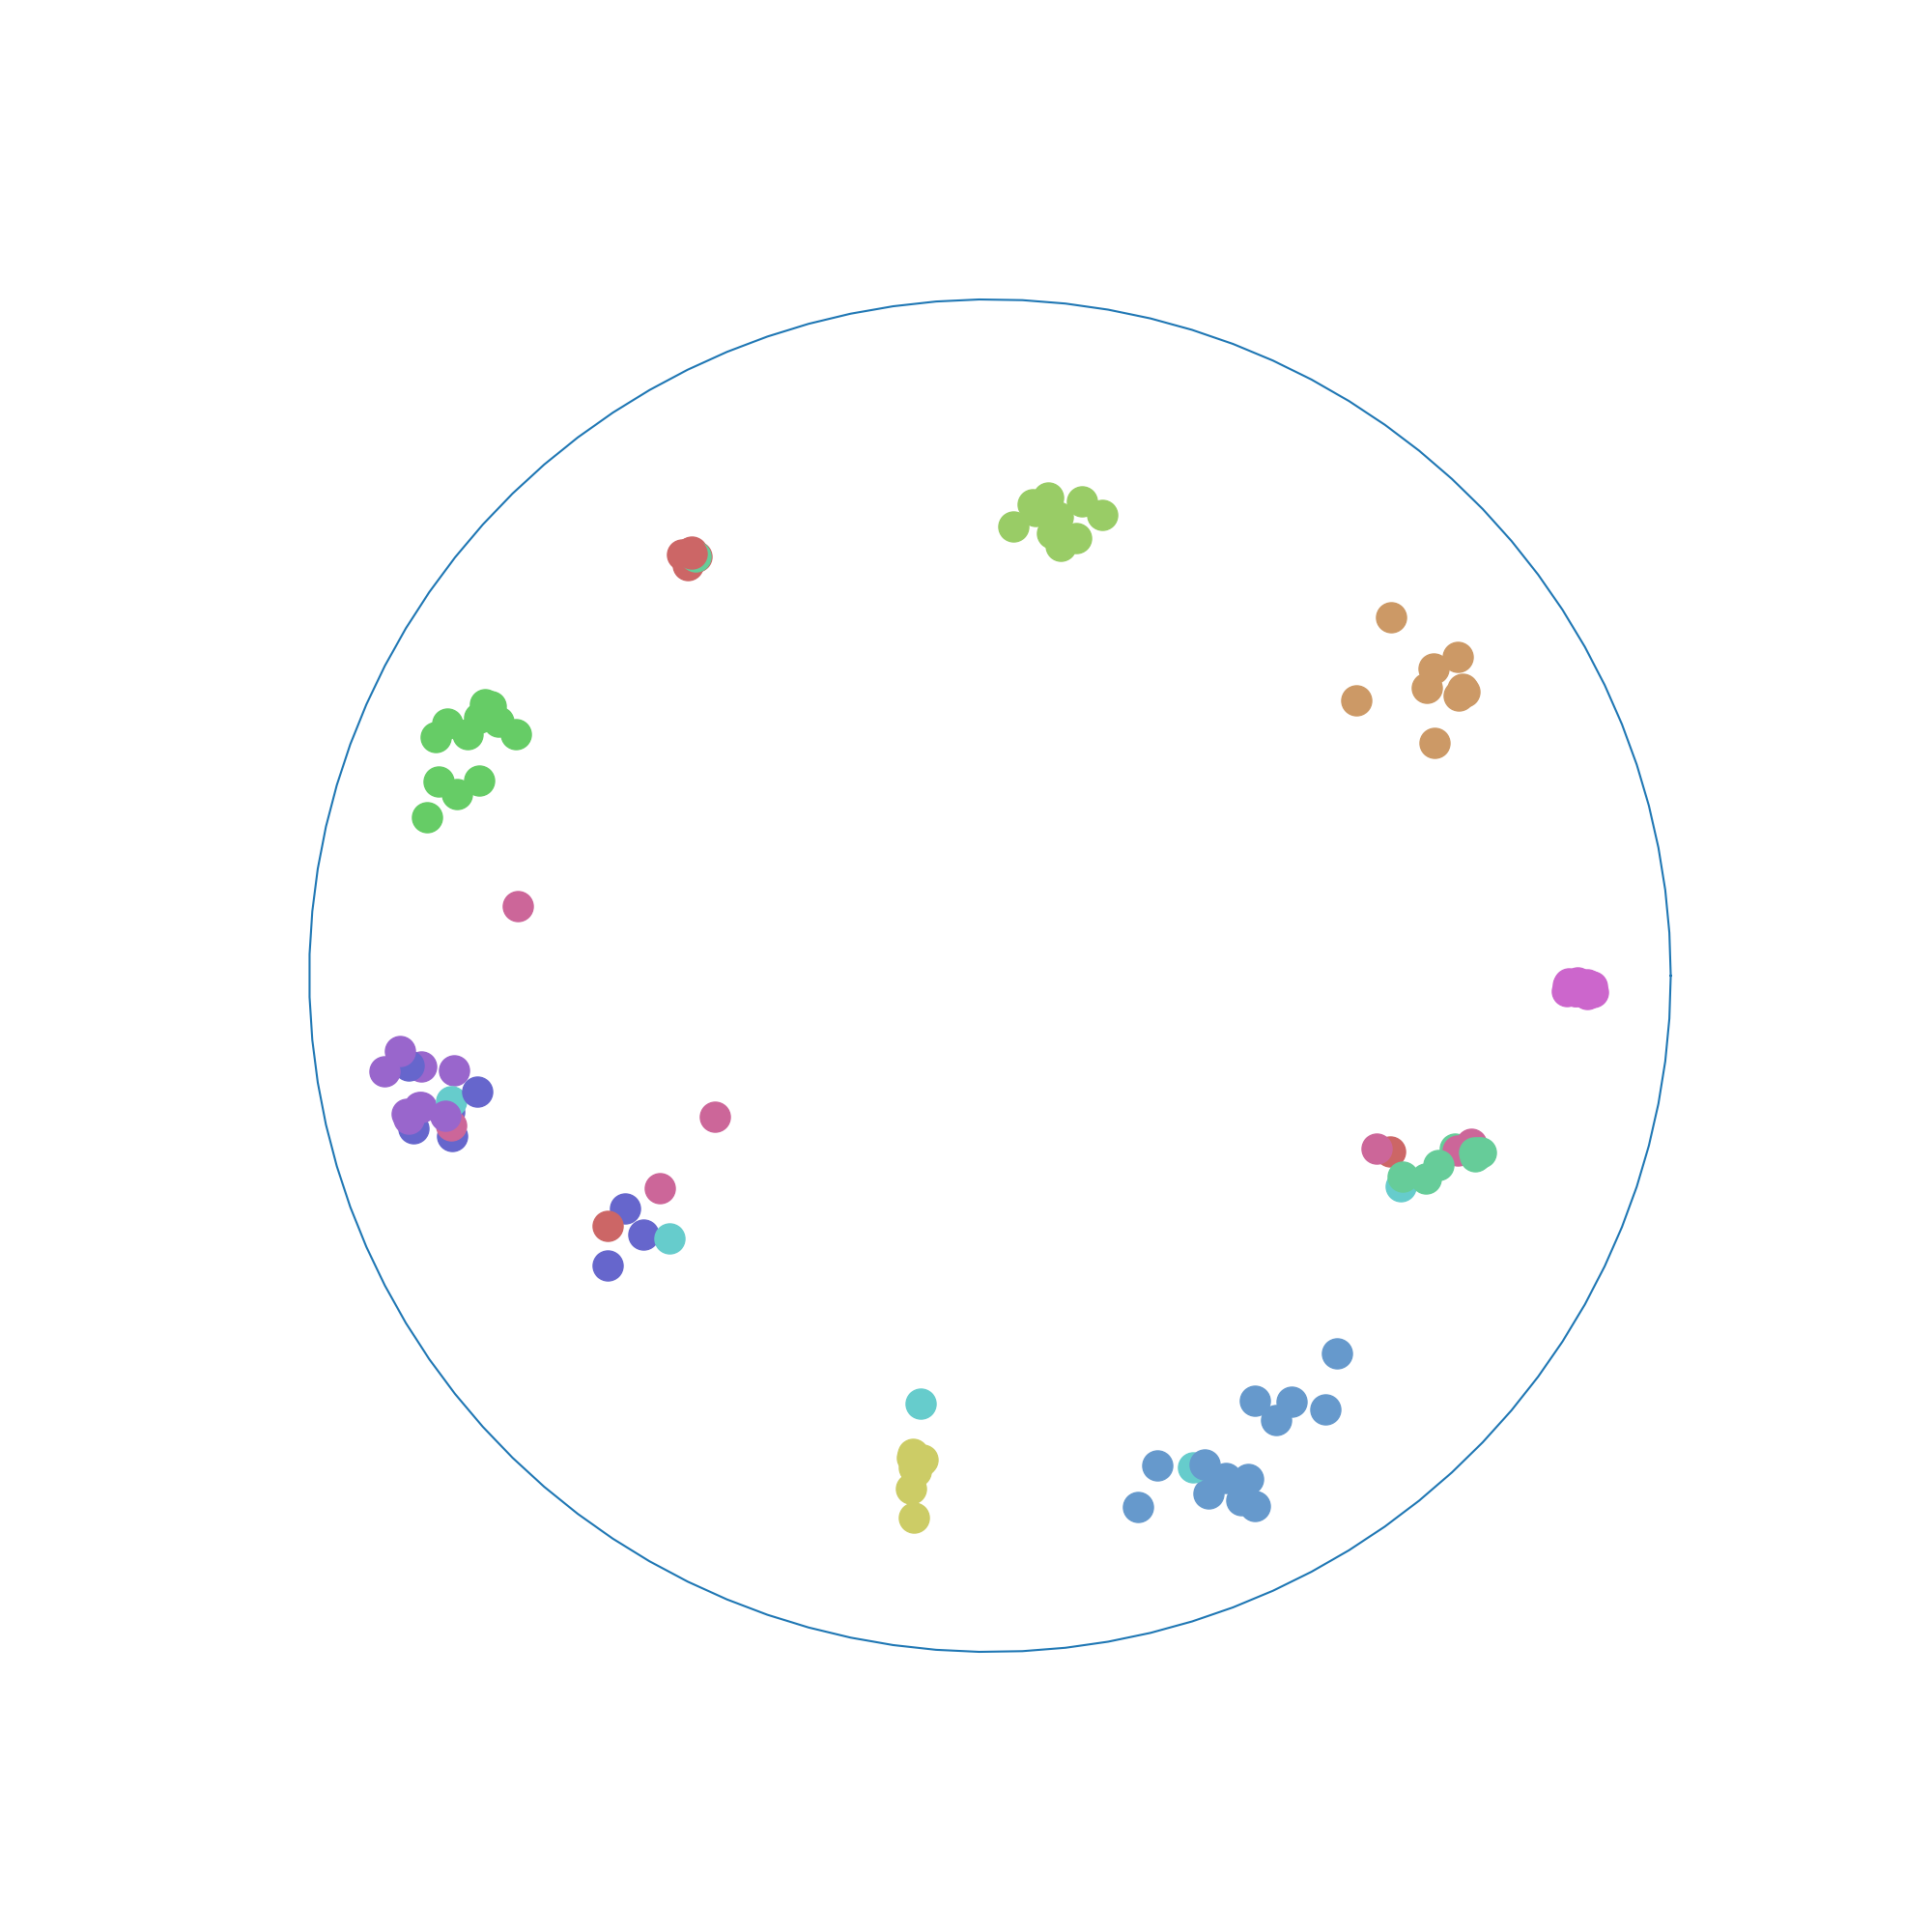
\includegraphics[scale=0.15]{media/embedding_barycenter_search.png}
                    \caption{Embeddings on which we performed the test}
                \end{subfigure}


                    \begin{tabular}{|c|c|}

                        \hline
                        Initialisation & Iterations to convergence \\
                        \hline
                        $\frac{1}{n}\sum \limits_{i=1}^n x_i$ & $428 \pm 6$  \\
                        $\frac{1}{\sum \limits_{j=1}^n w_{jk}}\sum \limits_{i=1}^n x_iw_{ik}$  & $133 \pm 62$ \\
                        \hline
                    \end{tabular}

            \end{figure}

    \section{Learning embeddings}
            \subsection{Batch, Mini-batch, sum or mean}

            \subsection{Negative sampling}

            \subsection{Compareason of optimization methods}

            \subsection{Going out of the ball border}
            
    \section{Parameters}:
        \begin{table}
            \centering
            \begin{tabular}{l|p{10cm}}
                \hline
                Parameter & Description \\
                --init-lr & Initial learning rate for the first epoch, before applying $O_3$ loss \\
                --lr & Learning rate applied on the gradient \\
                --init-alpha & $O_1$ loss weight for the first epoch (if not given is set to alpha value) \\
                --alpha & $O_1$ loss weitght \\
                --init-beta & $O_2$ loss weight for the first epoch (if not given is set to beta value) \\
                --beta & $O_2$ loss weight \\
                \hline
                \hline
                --gamma & $O_3$ loss weight (this loss is firstly applied at the second iteration/epoch) \\
                --n-gaussian & The number of gaussian in the gaussan mixture (mainly set to the number of community in the dataset) \\
                \hline
                --dataset & The dataset name in lowercase on which perform the experiment (see dataset section) \\
                \hline
                \hline
                --walk-lenght & The size of the random walk usually set to 20 \\
                --context-size & The size of the context, the window around each nodes in a path \\
                --precompute-rw & The number of path to consider from each nodes \\
                \hline
                \hline
                --negative-sampling & The number of negative examples for the $O_2$ loss (between 5 and 20) \\
                \hline
                \hline
                --epoch-embedding-init & The number of epoch (see all the nodes, couple on the graph) for the first embedding learning iteration, if not given is set to --epoch-embedding. We recommend to set more epoch for the first iteration than for others \\
                --epoch-embedding & The number of epoch for learning embedding\\
                \hline
                \hline
                --loss-aggregation & The type of aggregation of the loss must be "sum" or "mean". This paramaeters has a huge influence on the selection of learning rate and batch size. If choosing sum the learning rate must be low (between 1e-2 and 1e-4). If choosing mean the learning rate value must be high (from 1 to 10). \\
                --batch-size & the size of the batch (number of element to require grad without updating parameters). A small batch-size is recommended in order to have a small number of iteration, however large batch size will drastically lower the time of epoch. The default batch size is set to 10000 (on small dataset one batch allow to visit every examples). \\
                \hline


            \end{tabular}
        \end{table}
    \section{Dataset}
    \begin{table}
        \begin{tabular}{c|c|c|c}
            Dataset & \#nodes & \#edges &\#community \\
            karate & - & - & 2 \\
            poolblogs & -  & - & 2\\
            adjnoun & - & -& 2 \\
            poolbooks & - & - & 3\\
            football & - & - &  12 \\
            dblp & - & - & 5 \\
            
        \end{tabular}
    \end{table}
\end{document}